\documentclass{article}

\usepackage[main, final]{neurips_2026}

\usepackage[utf8]{inputenc} % allow utf-8 input
\usepackage[T1]{fontenc}    % use 8-bit T1 fonts
\usepackage{hyperref}       % hyperlinks
\usepackage{url}            % simple URL typesetting
\usepackage{booktabs}       % professional-quality tables
\usepackage{amsfonts}       % blackboard math symbols
\usepackage{nicefrac}       % compact symbols for 1/2, etc.
\usepackage{microtype}      % microtypography
\usepackage{xcolor}         % colors
\usepackage{float}
\usepackage{graphicx}
\usepackage{subcaption}
\usepackage{natbib}
\usepackage{amsmath, amssymb}
\usepackage{algorithm}
\usepackage{algpseudocode}
\usepackage{longtable}
\usepackage{array}
\usepackage{makecell}       % two-line table headers / cells
\usepackage{xurl}           % URLs may break anywhere
\usepackage{pdflscape}      % landscape pages for the widest appendix tables
\usepackage{etoolbox}
\usepackage{adjustbox}
% ---- Compact float layout (space for the analysis) -------------------------------------------------------
\usepackage[font=small,labelfont=bf,skip=3pt]{caption}
\setlength{\textfloatsep}{8pt plus 2pt minus 2pt}   % float above/below text
\setlength{\floatsep}{6pt plus 2pt minus 2pt}       % between two floats
\setlength{\intextsep}{6pt plus 2pt minus 2pt}
\renewcommand{\topfraction}{0.95}\renewcommand{\bottomfraction}{0.95}
\renewcommand{\textfraction}{0.05}\renewcommand{\floatpagefraction}{0.9}
\setcounter{topnumber}{4}\setcounter{bottomnumber}{4}\setcounter{totalnumber}{8}
% ---- Table style for every \input table: 8 pt text, tight columns and rows ----------------------------------
\AtBeginEnvironment{table}{%
  \setlength{\tabcolsep}{3.5pt}%
  \renewcommand{\arraystretch}{0.92}%
  \setlength{\aboverulesep}{1.5pt}\setlength{\belowrulesep}{1.5pt}%
  \renewcommand{\small}{\footnotesize}}
% Safety net: a table still wider than the line (or taller than the page) is scaled down to fit; never enlarged.
\let\oldtabular\tabular
\let\endoldtabular\endtabular
\renewenvironment{tabular}%
  {\begin{adjustbox}{max width=\linewidth, max totalheight=0.9\textheight}\oldtabular}%
  {\endoldtabular\end{adjustbox}}
\raggedbottom               % no stretched (underfull) pages around large floats
% Unicode symbols used in the generated tables
\DeclareUnicodeCharacter{2212}{\ensuremath{-}}
\DeclareUnicodeCharacter{2264}{\ensuremath{\leq}}
\DeclareUnicodeCharacter{03B3}{\ensuremath{\gamma}}
\DeclareUnicodeCharacter{03C4}{\ensuremath{\tau}}
\DeclareUnicodeCharacter{00B7}{\ensuremath{\cdot}}

% Placeholder marker: every TODO is text you still have to write.
\newcommand{\todo}[1]{\textcolor{red}{[TODO: #1]}}

\title{\todo{Title}}

\author{
  Faaiz Khan \\
  Syed Babar Ali School of Science and Engineering\\
  Lahore University of Management Sciences\\
  Lahore, Pakistan\\
  \texttt{25280051@lums.edu.pk} \\
}

\begin{document}

\maketitle
\suppressfloats[t]   % no floats above the title block

\begin{abstract}
  \todo{Abstract.}
  Code: \url{https://github.com/FaaizKhan1999/atml-assignment3}.
\end{abstract}

% =====================================================================================================
\section{Introduction}
\label{sec:intro}

\todo{Introduction.}

% =====================================================================================================
\section{Experimental Setup and Methods}
\label{sec:setup}

\subsection{Mathematical Fine-Tuning and Parameter-Restricted Adaptation}
\label{sec:setup-finetuning}

\todo{Setup and methods.}

\subsection{Vision-Language Interface and Grounding Evaluation}
\label{sec:setup-vlm}

\todo{Setup and methods.}

\subsection{Test-Time Compute: Sampling, Selection and Adaptive Inference}
\label{sec:setup-ttc}

\todo{Setup and methods.}

% =====================================================================================================
\section{Results and Analysis}
\label{sec:results}

% -----------------------------------------------------------------------------------------------------
\subsection{Specialization, Retention and Restrictions on Adaptation}
\label{sec:results-finetuning}

\todo{Analysis.}

% Benchmark results: all seven conditions x four benchmarks, change from baseline in pp.
\begin{table}[t]
\centering
\small
\caption{Zero-shot benchmark evaluation across mathematical and general reasoning tasks. Full-parameter fine-tuning and L2-SP achieve the largest in-domain mathematical gains alongside a raw BoolQ drop driven by a ``no'' prediction bias (while class-balanced BoolQ accuracy rises), whereas rank-16 LoRA and OPLoRA adapters deliver strong mathematical improvements and gain on BoolQ across both answer classes.}
\label{tab:t1-bench}
\begin{tabular}{lrrrrrrr}
\toprule
Condition & GSM8K (\%) & HellaSwag (\%) & BoolQ (\%) & ARC-E (\%) & Mean non-math $\Delta$pp & GSM8K unextr. \% & GSM8K trunc. \% \\
\midrule
Baseline & 43.4 & 47.3 & 64.4 & 56.0 & – & 0.0 & 0.8 \\
Full FT (mid) & 56.9 (+13.6) & 45.7 (-1.6) & 62.6 (-1.8) & 62.1 (+6.1) & +0.89 & 0.0 & 1.1 \\
Full FT & 64.4 (+21.0) & 45.9 (-1.4) & 61.5 (-2.8) & 63.7 (+7.7) & +1.14 & 0.0 & 0.2 \\
Full FT + L2-SP & 64.2 (+20.8) & 46.6 (-0.7) & 61.6 (-2.8) & 63.7 (+7.7) & +1.38 & 0.0 & 0.5 \\
LoRA-4 & 59.9 (+16.5) & 47.5 (+0.1) & 65.4 (+1.0) & 63.1 (+7.1) & +2.75 & 0.0 & 1.0 \\
LoRA-16 & 61.0 (+17.7) & 47.5 (+0.1) & 71.7 (+7.4) & 64.4 (+8.3) & +5.28 & 0.0 & 0.9 \\
OPLoRA-16 & 61.3 (+18.0) & 47.3 (+0.0) & 71.8 (+7.4) & 63.9 (+7.9) & +5.09 & 0.1 & 0.7 \\
\bottomrule
\end{tabular}
\end{table}


\begin{figure}[t]
  \centering
  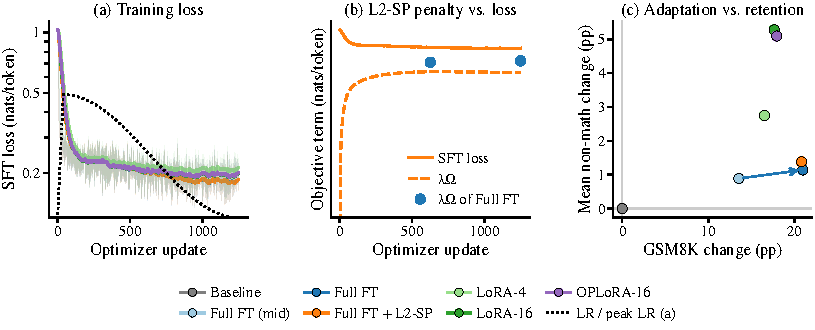
\includegraphics[width=0.82\textwidth]{figs/task1/fig1_training_tradeoff.pdf}
  \caption{\todo{Figure title.} \todo{1--2 sentences describing what is shown.} \todo{Conclusion to draw.}}
  \label{fig:ft-training-tradeoff}
\end{figure}

\todo{Analysis.}

% Resources and regularization: trainable parameters, time, memory, checkpoint sizes, displacement, penalty.
\begin{table}[t]
\centering
\small
\caption{Computational resource footprints, parameter efficiency, and weight-space displacement across fine-tuning regimes. Low-rank adaptation drastically reduces peak GPU memory and trainable parameter counts compared to full fine-tuning, though orthogonal projection introduces additional training latency and subspace precomputation overheads.}
\label{tab:t1-resources}
\begin{tabular}{lrrrrrl}
\toprule
Method & \makecell{Trainable\\params} & \makecell{Train\\time (h)} & \makecell{Peak GPU\\mem. (GB)} & \makecell{Exported\\weights} & $\|\theta-\theta_0\|_2$ & Method-specific overhead \\
\midrule
Full FT & 596.05M (100.00\%) & 2.36 & 11.95 & 2.22 GB & 10.65 & – \\
Full FT + L2-SP & 596.05M (100.00\%) & 2.46 & 11.95 & 2.22 GB & 6.26 & $\theta_0$ copy 2.22 GB (CPU); penalty 5.6 min \\
LoRA-4 & 2.52M (0.42\%) & 2.68 & 3.14 & 9.7 MB & – & – \\
LoRA-16 & 10.09M (1.67\%) & 2.63 & 3.25 & 38.5 MB & – & – \\
OPLoRA-16 & 10.09M (1.67\%) & 3.50 & 3.56 & 346.6 MB & – & SVD+QR 39 s; bases 308.0 MB \\
\bottomrule
\end{tabular}
\end{table}


\begin{figure}[t]
  \centering
  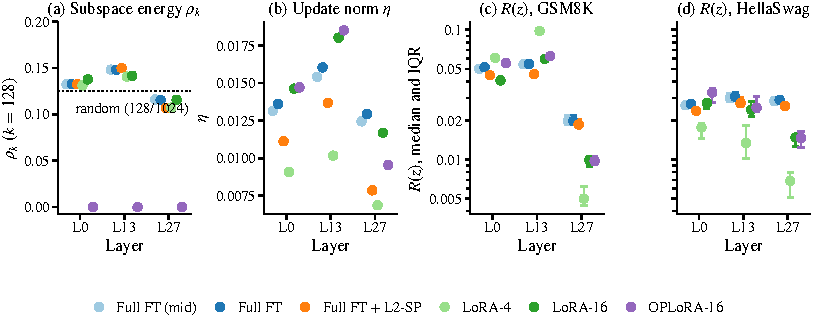
\includegraphics[width=0.68\textwidth]{figs/task1/fig2_diagnostics.pdf}
  \caption{\todo{Figure title.} \todo{1--2 sentences describing what is shown.} \todo{Conclusion to draw.}}
  \label{fig:ft-diagnostics}
\end{figure}

\todo{Analysis.}

% Qualitative findings: summary of the 42 annotated responses (aligned excerpts: Appendix, Table in app:ft-excerpts).
\begin{table}[t]
\centering
\small
\caption{Qualitative human evaluation of generation coherence, formatting compliance, and failure modes across a small response sample. Unconstrained full fine-tuning reduces mean coherence by introducing severe repetition and unprompted mathematical framing, whereas L2-SP avoids severe repetition and low-rank adapters improve coherence while largely avoiding mathematical framing on general prompts, with zero inappropriate content observed across all conditions.}
\label{tab:t1-annotation}
\begin{tabular}{lrrrrrr}
\toprule
Condition & \makecell{Format:\\yes/partial/no} & \makecell{Mean coherence\\(1–3)} & \makecell{Repetition:\\some/severe} & Math framing & Truncated & Inappropriate \\
\midrule
Baseline & 2/2/2 & 2.33 & 0/0 & 0/6 & 0/6 & 0/6 \\
Full FT (mid) & 2/2/2 & 1.83 & 2/2 & 4/6 & 2/6 & 0/6 \\
Full FT & 3/2/1 & 2.17 & 3/2 & 3/6 & 2/6 & 0/6 \\
Full FT + L2-SP & 3/2/1 & 2.17 & 3/0 & 4/6 & 0/6 & 0/6 \\
LoRA-4 & 3/1/2 & 2.50 & 0/1 & 0/6 & 0/6 & 0/6 \\
LoRA-16 & 3/2/1 & 2.50 & 2/1 & 0/6 & 1/6 & 0/6 \\
OPLoRA-16 & 3/1/2 & 2.67 & 1/0 & 1/6 & 0/6 & 0/6 \\
\bottomrule
\end{tabular}
\end{table}


\todo{Analysis.}

% -----------------------------------------------------------------------------------------------------
\subsection{Learning a Visual Interface and Measuring Visual Grounding}
\label{sec:results-vlm}

\todo{Analysis.}

\begin{figure}[t]
  \centering
  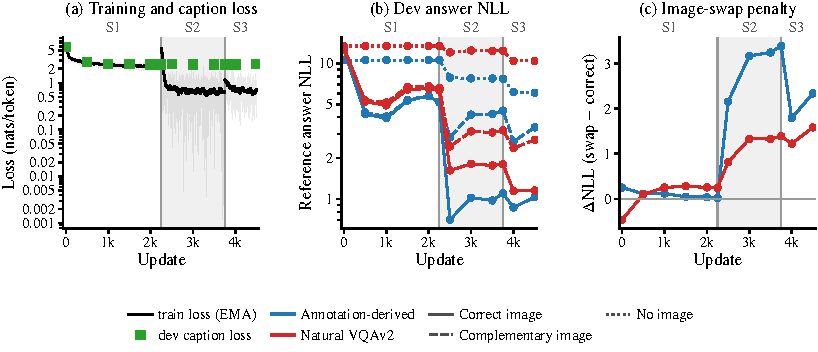
\includegraphics[width=0.74\textwidth]{figs/task2/fig1_learning_curves.pdf}
  \caption{\todo{Figure title.} \todo{1--2 sentences describing what is shown.} \todo{Conclusion to draw.}}
  \label{fig:vlm-learning-curves}
\end{figure}

\todo{Analysis.}

% Final results: both suites x four image conditions, question types, pair diagnostics, NLL, bootstrap CIs.
\begin{table}[t]
\centering
\small
\caption{Final stage-three evaluation under correct, complementary, mismatched, and no-image conditions. The model achieves its highest accuracy and lowest answer loss with the correct image compared to complementary or mismatched inputs, while removing the image causes the model to generate identical full-sentence responses per prompt, which reduces strict exact-match accuracy far more than lead-answer accuracy.}
\label{tab:t2-final}
\begin{tabular}{llrrrrrr}
\toprule
Suite & Image & \makecell{Accuracy \%\\{}[95\% CI]} & \makecell{Pair\\acc. \%} & \makecell{Identical\\\%} & \makecell{Ref.\\NLL} & \makecell{ms /\\answer} & \makecell{Lead-\\ans. \%$^\dagger$} \\
\midrule
Annotation-derived & Correct & 66.4 [57.0, 75.0] & 50.0 & 20.3 & 0.93 & 42 & 66.4 \\
(64 pairs) & Complementary & 10.9 [6.2, 16.4] & 0.0 & 20.3 & 4.02 & 30 & 10.9 \\
 & Mismatched & 37.5 [30.5, 45.3] & 9.4 & 64.1 & 2.38 & 30 & 37.5 \\
 & No image & 0.0 [0.0, 0.0] & 0.0 & 100.0 & 6.55 & 111 & 25.0 \\
\midrule
Natural VQAv2 & Correct & 56.6 [50.0, 63.1] & 27.1 & 40.6 & 1.40 & 35 & 55.9 \\
(96 pairs) & Complementary & 27.1 [20.9, 33.5] & 5.2 & 40.6 & 2.85 & 35 & 36.5 \\
 & Mismatched & 35.4 [29.1, 42.1] & 8.3 & 56.2 & 2.34 & 39 & 47.0 \\
 & No image & 1.0 [0.0, 2.6] & 0.0 & 100.0 & 9.52 & 123 & 29.2 \\
\bottomrule
\end{tabular}
\end{table}


\begin{figure}[t]
  \centering
  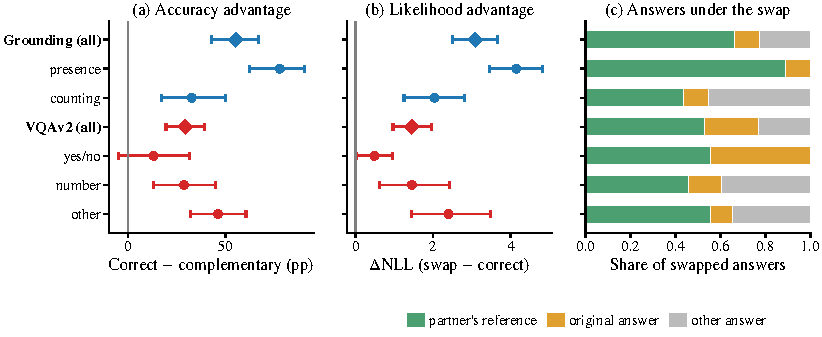
\includegraphics[width=0.8\textwidth]{figs/task2/fig2_image_use.pdf}
  \caption{\todo{Figure title.} \todo{1--2 sentences describing what is shown.} \todo{Conclusion to draw.}}
  \label{fig:vlm-image-use}
\end{figure}

\todo{Analysis.}

\begin{figure}[t]
  \centering
  % the PDF's blank band between its two rows of examples (y = 110--154 pt of 266 pt) is trimmed out
  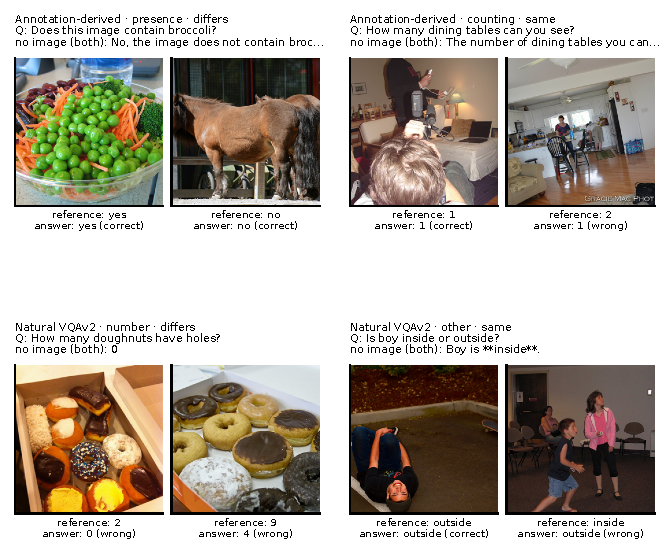
\includegraphics[width=0.62\textwidth,trim={0 153 0 4},clip]{figs/task2/fig3_qualitative.pdf}\\[2pt]
  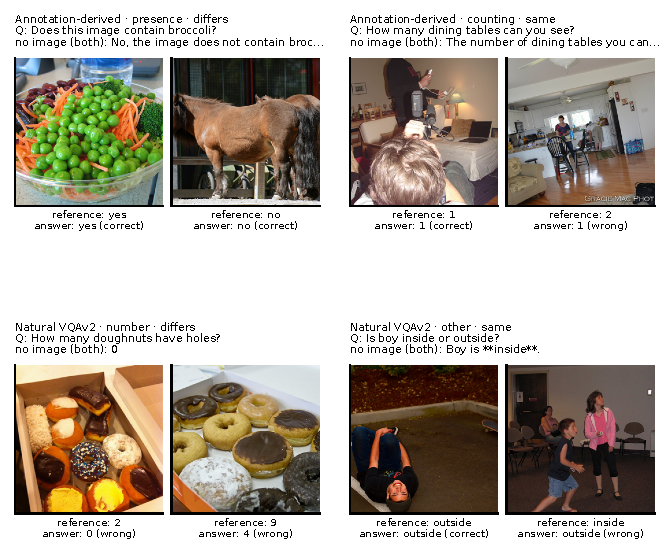
\includegraphics[width=0.62\textwidth,trim={0 6 0 150},clip]{figs/task2/fig3_qualitative.pdf}
  \caption{\todo{Figure title.} \todo{1--2 sentences describing what is shown, including the example-selection rule.} \todo{Conclusion to draw.}}
  \label{fig:vlm-qualitative}
\end{figure}


\todo{Analysis.}

% -----------------------------------------------------------------------------------------------------
\subsection{Allocating Test-Time Compute: Sampling, Selection and Stopping}
\label{sec:results-ttc}

\todo{Analysis.}

\begin{figure}[t]
  \centering
  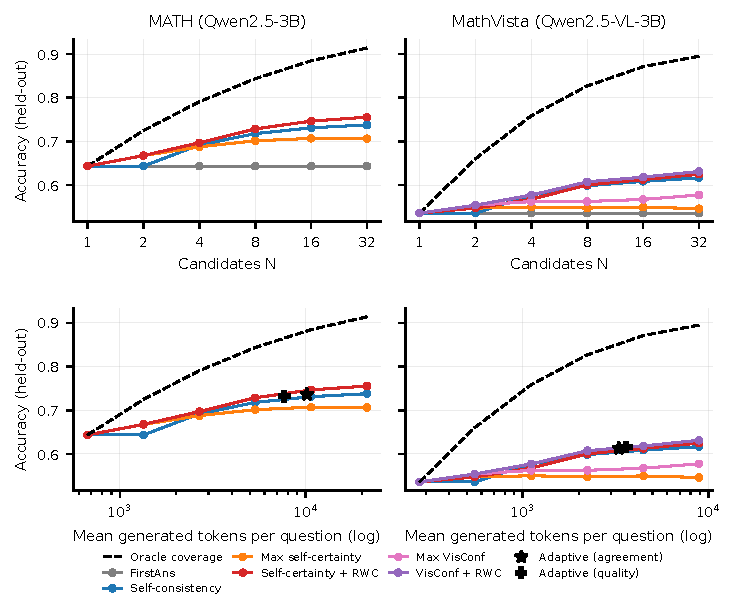
\includegraphics[width=0.56\textwidth]{figs/task3/fig1_compute_curves.pdf}
  \caption{\todo{Figure title.} \todo{1--2 sentences describing what is shown.} \todo{Conclusion to draw.}}
  \label{fig:ttc-compute-curves}
\end{figure}

% Compact method comparison at N = 8 and N = 32.
\begin{table}[t]
\centering
\small
\caption{Held-out accuracy (\%) of each selection rule (800 questions per dataset; averaged over ten rollout orders, then questions). $\Delta$: paired question-level bootstrap (1,000 resamples) of the difference from self-consistency at N = 32. Tokenwise rows are the fusion ablation (confidence $\times$ vision per token); the shortest-rollout rule is a length-only control. Oracle coverage uses reference answers and is not a method.}
\label{tab:t3-methods}
\begin{tabular}{>{\raggedright\arraybackslash}p{3.4cm}rrrrrr}
\toprule
Method & MATH N=8 & MATH N=32 & \makecell{MATH $\Delta$ vs\\SC @32 [95\% CI]} & \makecell{MathVista\\N=8} & \makecell{MathVista\\N=32} & \makecell{MathVista $\Delta$\\vs SC @32 [95\% CI]} \\
\midrule
FirstAns & 64.4 & 64.4 & -9.4 [-11.1, -7.8] & 53.6 & 53.6 & -8.1 [-10.0, -6.2] \\
Self-consistency & 71.8 & 73.8 & – & 59.9 & 61.7 & – \\
Max mean log-prob & 67.5 & 64.0 & -9.8 [-12.4, -7.2] & 51.9 & 48.1 & -13.6 [-17.0, -10.3] \\
Max self-certainty & 70.1 & 70.6 & -3.2 [-5.6, -0.8] & 54.8 & 54.6 & -7.1 [-10.2, -3.8] \\
Self-certainty + RWC & 72.9 & 75.5 & +1.8 [+0.7, +2.8] & 60.0 & 62.5 & +0.8 [-0.6, +2.1] \\
Shortest (length control) & 64.6 & 62.4 & -11.4 [-14.1, -9.0] & 54.6 & 53.8 & -7.8 [-11.0, -4.9] \\
Max vision & – & – & – & 54.3 & 53.6 & -8.1 [-11.3, -4.9] \\
Vision + RWC & – & – & – & 60.1 & 62.9 & +1.2 [-0.3, +2.8] \\
Max VisConf & – & – & – & 56.3 & 57.8 & -3.9 [-7.0, -0.9] \\
VisConf + RWC & – & – & – & 60.8 & 63.1 & +1.4 [+0.0, +3.0] \\
Max VisConf (tokenwise) & – & – & – & 55.7 & 56.2 & -5.4 [-8.4, -2.4] \\
VisConf tokenwise + RWC & – & – & – & 60.9 & 62.6 & +1.0 [-0.4, +2.4] \\
Oracle coverage (upper bound) & 84.3 & 91.4 & – & 82.7 & 89.5 & – \\
\bottomrule
\end{tabular}
\end{table}


\todo{Analysis.}

\begin{figure}[t]
  \centering
  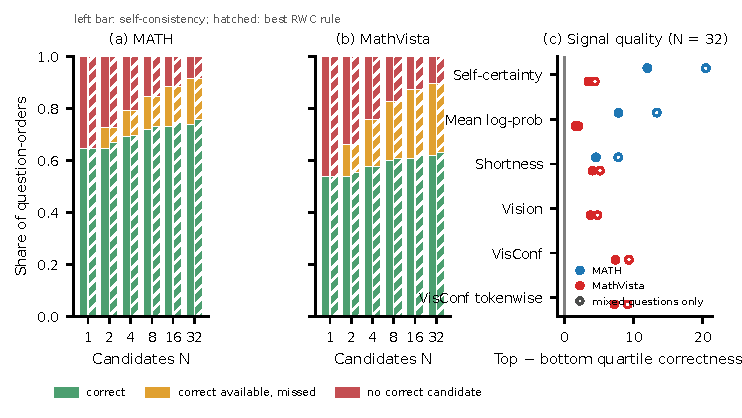
\includegraphics[width=0.74\textwidth]{figs/task3/fig2_failures_signals.pdf}
  \caption{\todo{Figure title.} \todo{1--2 sentences describing what is shown.} \todo{Conclusion to draw.}}
  \label{fig:ttc-failures-signals}
\end{figure}


\todo{Analysis.}

% Live inference: single response vs parallel sampling vs sequential refinement.
\begin{table}[t]
\centering
\small
\caption{End-to-end latency, token overhead, and accuracy for live single-pass, parallel, and iterative refinement decoding. Under strict generation budgets, naive parallel sampling and multi-turn self-revision increase computational latency and truncation rates without improving accuracy, as beneficial revisions are offset by self-induced corruptions.}
\label{tab:t3-live}
\begin{tabular}{lrrrrrrr}
\toprule
Strategy & Acc. \% & \makecell{$\Delta$ vs single\\[95\% CI]} & \makecell{Input\\tokens} & \makecell{Output\\tokens} & \makecell{Total\\tokens} & \makecell{s /\\question} & \makecell{Truncated\\calls \%} \\
\midrule
Single ($\leq$3,072) & 66.0 & – & 108 & 734 & 843 & 36.5 & 4.0 \\
Parallel $\times$3 + SC & 62.0 & -4 [-16, +6] & 325 & 1821 & 2146 & 89.2 & 16.0 \\
Refinement & 64.0 & -2 [-12, +10] & 837 & 1117 & 1955 & 55.4 & 5.0 \\
\bottomrule
\end{tabular}
\end{table}


\todo{Analysis.}

% Adaptive inference: development-selected thresholds and held-out accuracy-cost results.
\begin{table}[t]
\centering
\small
\caption{Performance and stopping distributions of agreement- and quality-based adaptive early-stopping policies. Both adaptive policies halt at the minimum rollout threshold on a majority of question-order instances to cut average rollout counts by more than half, showing no statistically significant accuracy loss relative to full-budget voting except for a small drop under the quality-aware policy on MATH.}
\label{tab:t3-adaptive}
\begin{tabular}{llllrrrl}
\toprule
Dataset & Policy & \makecell{Setting\\(dev)} & Accuracy \% & \makecell{$\Delta$ vs\\SC@32 [95\% CI]} & Tokens / q. & Rollouts & \makecell{Stops at 4 / 8\\/ 16 / 32 (\%)} \\
\midrule
MATH & Fixed SC, N = 4 & – & 69.2 & – & 2680 & 4 & – \\
 & Fixed SC, N = 8 & – & 71.8 & – & 5344 & 8 & – \\
 & Fixed SC, N = 16 & – & 73.1 & – & 10678 & 16 & – \\
 & Fixed SC, N = 32 & – & 73.8 & – & 21347 & 32 & – \\
 & Adaptive: agreement & τ = 0.625 & 73.6 & -0.1 [-0.5, +0.2] & 10140 & 11.8 & 66 / 6 / 1 / 27 \\
 & Adaptive: quality & τ = 0.5, γ = 0.0 & 73.2 & -0.6 [-1.2, -0.1] & 7663 & 9.0 & 76 / 6 / 1 / 16 \\
\midrule
MathVista & Fixed SC, N = 4 & – & 57.8 & – & 1112 & 4 & – \\
 & Fixed SC, N = 8 & – & 59.9 & – & 2230 & 8 & – \\
 & Fixed SC, N = 16 & – & 60.9 & – & 4462 & 16 & – \\
 & Fixed SC, N = 32 & – & 61.7 & – & 8898 & 32 & – \\
 & Adaptive: agreement & τ = 0.5 & 61.3 & -0.4 [-1.6, +0.7] & 3290 & 9.9 & 71 / 8 / 2 / 19 \\
 & Adaptive: quality & τ = 0.5, γ = 0.0 & 61.6 & -0.1 [-1.1, +0.9] & 3613 & 10.9 & 65 / 10 / 3 / 22 \\
\bottomrule
\end{tabular}
\end{table}


\todo{Analysis.}

% Qualitative findings: selection disagreement, revision, premature stopping.
\begin{table}[t]
\centering
\small
\caption{Qualitative failure and success cases across confidence-weighted voting, iterative revision, and adaptive stopping. Every test-time scaling mechanism exhibits distinct vulnerabilities—including overconfident misselection, successful format recovery during revision, and premature convergence on shared errors—highlighting the complementary limits of aggregation, refinement, and early stopping.}
\label{tab:t3-examples}
\begin{tabular}{>{\raggedright\arraybackslash}p{3.4cm}l>{\raggedright\arraybackslash}p{8.2cm}}
\toprule
Behaviour & Question & \makecell{What\\happened} \\
\midrule
Selection disagreement (MathVista, N = 32, order 0) & 552 & SC $\to$ 4 (correct); VisConf + RWC $\to$ 2 (wrong) \\
Revision changes correctness (live MATH) & test:2340 & initial None (wrong) $\to$ revised 6 (correct); gold 6 \\
Premature stop (MATH, quality-aware) & test:3504 & stopped after 4 with 120 (wrong); fixed-32 SC would be correct (order 7) \\
\bottomrule
\end{tabular}
\end{table}


\todo{Analysis.}

% =====================================================================================================
\section{Conclusion}
\label{sec:conclusion}

\todo{Conclusion.}

\clearpage

{
\small
\bibliographystyle{unsrtnat}
\nocite{*}
\bibliography{refs}
}

\clearpage

\appendix

% =====================================================================================================
\section{Mathematical Fine-Tuning: Supplementary Results}
\label{app:finetuning}

\subsection{Training Data Selection}
\label{app:ft-data}
\todo{Text.}
\begin{table}[t]
\centering
\small
\caption{MetaMathQA selection. Normalization for decontamination: NFKC; lowercase; runs of [\^{}0-9a-z] -> single space; strip.}
\label{tab:t1-data}
\begin{tabular}{>{\raggedright\arraybackslash}p{3.4cm}r}
\toprule
Item & Value \\
\midrule
Rows scanned (source order) & 40,002 \\
Selected examples & 40,000 \\
Excluded: too long & 2 \\
GSM8K test questions checked (normalized) & 1,319 \\
Responses with leading newlines stripped & 667 \\
Input tokens (total) & 9.91M \\
Supervised tokens (total) & 7.10M \\
Formatted length mean / p99 / max & 248 / 681 / 1941 \\
Template render mismatches & 0 \\
\bottomrule
\end{tabular}
\end{table}


\subsection{Complete Benchmark Metrics}
\label{app:ft-bench}
\todo{Text.}
\begin{table}[t]
\centering
\small
\caption{All benchmark metrics (\%, $\pm$ lm-eval standard error). Raw accuracy is reported alongside normalized accuracy; GSM8K strict-match requires the “The answer is” format.}
\label{tab:t1-bench-full}
\begin{tabular}{lrrrrrrrr}
\toprule
Condition & GSM8K flex & GSM8K strict & GSM8K mean tokens & HellaSwag acc\_norm & HellaSwag acc & BoolQ acc & ARC-E acc\_norm & ARC-E acc \\
\midrule
Baseline & 43.4 $\pm$ 1.4 & 0.0 $\pm$ 0.0 & 226 & 47.3 $\pm$ 0.5 & 37.5 $\pm$ 0.5 & 64.4 $\pm$ 0.8 & 56.0 $\pm$ 1.0 & 60.9 $\pm$ 1.0 \\
Full FT (mid) & 56.9 $\pm$ 1.4 & 0.0 $\pm$ 0.0 & 143 & 45.7 $\pm$ 0.5 & 37.2 $\pm$ 0.5 & 62.6 $\pm$ 0.8 & 62.1 $\pm$ 1.0 & 66.2 $\pm$ 1.0 \\
Full FT & 64.4 $\pm$ 1.3 & 0.0 $\pm$ 0.0 & 136 & 45.9 $\pm$ 0.5 & 37.4 $\pm$ 0.5 & 61.5 $\pm$ 0.9 & 63.7 $\pm$ 1.0 & 67.0 $\pm$ 1.0 \\
Full FT + L2-SP & 64.2 $\pm$ 1.3 & 0.0 $\pm$ 0.0 & 138 & 46.6 $\pm$ 0.5 & 37.5 $\pm$ 0.5 & 61.6 $\pm$ 0.9 & 63.7 $\pm$ 1.0 & 66.3 $\pm$ 1.0 \\
LoRA-4 & 59.9 $\pm$ 1.4 & 0.0 $\pm$ 0.0 & 142 & 47.5 $\pm$ 0.5 & 37.6 $\pm$ 0.5 & 65.4 $\pm$ 0.8 & 63.1 $\pm$ 1.0 & 65.3 $\pm$ 1.0 \\
LoRA-16 & 61.0 $\pm$ 1.3 & 0.0 $\pm$ 0.0 & 143 & 47.5 $\pm$ 0.5 & 37.9 $\pm$ 0.5 & 71.7 $\pm$ 0.8 & 64.4 $\pm$ 1.0 & 66.8 $\pm$ 1.0 \\
OPLoRA-16 & 61.3 $\pm$ 1.3 & 0.0 $\pm$ 0.0 & 139 & 47.3 $\pm$ 0.5 & 37.8 $\pm$ 0.5 & 71.8 $\pm$ 0.8 & 63.9 $\pm$ 1.0 & 66.9 $\pm$ 1.0 \\
\bottomrule
\end{tabular}
\end{table}


\subsection{Yes/No Answer Balance on Reading Comprehension}
\label{app:ft-boolq}
\todo{Text.}
\begin{table}[t]
\centering
\small
\caption{BoolQ answer balance (validation, 3,270 questions; gold “yes” share 62.2\%). Predictions are the higher-likelihood choice; balanced accuracy averages accuracy over gold-yes and gold-no questions.}
\label{tab:t1-boolq}
\begin{tabular}{lrrrrr}
\toprule
Condition & Predicts “yes” (\%) & Acc. on gold-yes (\%) & Acc. on gold-no (\%) & Balanced acc. (\%) & Acc. (\%) \\
\midrule
Baseline & 57.7 & 67.8 & 58.8 & 63.3 & 64.4 \\
Full FT (mid) & 33.9 & 47.2 & 88.0 & 67.6 & 62.6 \\
Full FT & 31.5 & 44.4 & 89.7 & 67.1 & 61.5 \\
Full FT + L2-SP & 32.9 & 45.5 & 87.9 & 66.7 & 61.6 \\
LoRA-4 & 43.4 & 57.1 & 79.1 & 68.1 & 65.4 \\
LoRA-16 & 57.7 & 73.7 & 68.6 & 71.1 & 71.7 \\
OPLoRA-16 & 54.8 & 71.4 & 72.4 & 71.9 & 71.8 \\
\bottomrule
\end{tabular}
\end{table}


\subsection{Weight-Space and Activation Diagnostics}
\label{app:ft-diagnostics}
\todo{Text.}
\begin{table}[t]
\centering
\small
\caption{down\_proj diagnostics (FP32; k = 128; random-direction reference $\rho_k$ = k/d\_out = 0.125). For OPLoRA, parentheses give $\rho_k$ with its own training bases (numerical check of the projection). R over 32 GSM8K and 32 HellaSwag probe prompts.}
\label{tab:t1-diag-full}
\begin{tabular}{lrrrrrrrr}
\toprule
Condition & Layer & ρk & ρk (input) & η & ‖$\Delta$W‖F & R math median & R non-math median & Median ratio \\
\midrule
Full FT (mid) & 0 & 0.1325 & 0.0464 & 0.0132 & 0.612 & 0.0500 & 0.0263 & 1.90 \\
Full FT (mid) & 13 & 0.1482 & 0.0404 & 0.0154 & 0.656 & 0.0542 & 0.0298 & 1.82 \\
Full FT (mid) & 27 & 0.1161 & 0.0528 & 0.0125 & 0.596 & 0.0199 & 0.0283 & 0.70 \\
Full FT & 0 & 0.1324 & 0.0463 & 0.0136 & 0.634 & 0.0515 & 0.0269 & 1.92 \\
Full FT & 13 & 0.1481 & 0.0404 & 0.0160 & 0.683 & 0.0546 & 0.0305 & 1.79 \\
Full FT & 27 & 0.1155 & 0.0521 & 0.0130 & 0.620 & 0.0198 & 0.0288 & 0.69 \\
Full FT + L2-SP & 0 & 0.1325 & 0.0462 & 0.0111 & 0.518 & 0.0446 & 0.0238 & 1.88 \\
Full FT + L2-SP & 13 & 0.1499 & 0.0388 & 0.0137 & 0.583 & 0.0455 & 0.0272 & 1.67 \\
Full FT + L2-SP & 27 & 0.1068 & 0.0425 & 0.0079 & 0.376 & 0.0186 & 0.0259 & 0.72 \\
LoRA-4 & 0 & 0.1313 & 0.0444 & 0.0091 & 0.423 & 0.0609 & 0.0177 & 3.45 \\
LoRA-4 & 13 & 0.1407 & 0.0397 & 0.0102 & 0.433 & 0.0979 & 0.0135 & 7.27 \\
LoRA-4 & 27 & 0.1073 & 0.0404 & 0.0069 & 0.329 & 0.0050 & 0.0069 & 0.73 \\
LoRA-16 & 0 & 0.1376 & 0.0450 & 0.0146 & 0.681 & 0.0408 & 0.0273 & 1.49 \\
LoRA-16 & 13 & 0.1416 & 0.0414 & 0.0180 & 0.768 & 0.0599 & 0.0242 & 2.47 \\
LoRA-16 & 27 & 0.1156 & 0.0428 & 0.0117 & 0.560 & 0.0099 & 0.0148 & 0.67 \\
OPLoRA-16 & 0 & 0.0000 (9.5e-15) & 0.0000 & 0.0147 & 0.685 & 0.0554 & 0.0329 & 1.68 \\
OPLoRA-16 & 13 & 0.0000 (9.1e-15) & 0.0000 & 0.0185 & 0.788 & 0.0625 & 0.0251 & 2.49 \\
OPLoRA-16 & 27 & 0.0000 (9.9e-15) & 0.0000 & 0.0095 & 0.457 & 0.0098 & 0.0147 & 0.66 \\
\bottomrule
\end{tabular}
\end{table}


\subsection{Numerical Verification of Merging and Orthogonal Projection}
\label{app:ft-verification}
\todo{Text.}
\begin{table}[t]
\centering
\small
\caption{Numerical checks (separate from benchmark evidence). Merge check on 4 training sequences: merged FP16 model vs. unmerged adapter model, with the merge error relative to the adapter's own effect (unmerged vs. base). OPLoRA constraint residuals of the exported projected factors.}
\label{tab:t1-verify}
\begin{tabular}{lrrrrr}
\toprule
Method & Merged vs. unmerged: argmax agree (\%) & Mean |$\Delta$logit| merge / adapter effect & Max rel. ‖Uk\^{}T B\textasciitilde{}‖ & Max rel. ‖A\textasciitilde{} Vk‖ & Basis ortho. error (SVD $\to$ QR) \\
\midrule
LoRA-4 & 100.00 & 0.0050 & – & – & – \\
LoRA-16 & 99.87 & 0.0049 & – & – & – \\
OPLoRA-16 & 100.00 & 0.0047 & 1.1e-07 & 1.0e-07 & 4.3e-05 $\to$ 6.0e-07 \\
\bottomrule
\end{tabular}
\end{table}


\subsection{Automatic Checks on All Qualitative Prompts}
\label{app:ft-autoflags}
\todo{Text.}
\begin{table}[t]
\centering
\small
\caption{Automatic checks over all 24 qualitative prompts (8 questions × 3 formats) per condition. Math markers include LaTeX, equations, “The answer is” and “\#\#\#\#”. Template keys complete: every non-optional key filled with a value other than the template's placeholder.}
\label{tab:t1-autoflags}
\begin{tabular}{lrrrrrr}
\toprule
Condition & \makecell{Truncated\\/24} & \makecell{JSON valid\\as-is /8} & \makecell{JSON valid after\\unfencing /8} & \makecell{Template keys\\complete /8} & \makecell{With math\\markers /24} & \makecell{Mean repeated-line\\fraction} \\
\midrule
Baseline & 1 & 0 & 8 & 4 & 0 & 0.053 \\
Full FT (mid) & 6 & 2 & 2 & 7 & 15 & 0.176 \\
Full FT & 7 & 2 & 2 & 7 & 12 & 0.199 \\
Full FT + L2-SP & 2 & 2 & 2 & 7 & 13 & 0.038 \\
LoRA-4 & 1 & 3 & 3 & 6 & 2 & 0.052 \\
LoRA-16 & 4 & 3 & 3 & 6 & 4 & 0.069 \\
OPLoRA-16 & 3 & 3 & 3 & 6 & 9 & 0.048 \\
\bottomrule
\end{tabular}
\end{table}


\subsection{Annotated Excerpts}
\label{app:ft-excerpts}
\todo{Text.}
\begin{table}[t]
\centering
\small
\caption{Aligned excerpts: “enough\_of\_my\_husband” (template format), same prompt across all conditions.}
\label{tab:t1-excerpts}
\begin{tabular}{lcc>{\raggedright\arraybackslash}p{7.2cm}}
\toprule
Condition & Format & Coherence & Excerpt \\
\midrule
Baseline & yes & 3 & idea\_1 = I will start by discussing our feelings and understanding each other better. \\
Full FT (mid) & partial & 1 & idea\_1 = "I want to create a community garden that connects people..." \\
Full FT & partial & 2 & idea\_1 = "I want to help my husband with his daily tasks" ... The answer is: \\
Full FT + L2-SP & partial & 2 & idea\_3 = "I want to create a new hobby..." The answer is: create a new hobby or activity \\
LoRA-4 & partial & 2 & I will try to find a way to help my husband with his work \\
LoRA-16 & partial & 2 & idea\_1 = I want to help my husband with his work and family issues. \\
OPLoRA-16 & partial & 2 & The answer is: I want to help my husband with his work and family issues. \\
\bottomrule
\end{tabular}
\end{table}

% Long table: may need to be split or converted to longtable if it overflows the page.
\begin{table}[t]
\centering
\small
\caption{All annotated excerpts (42 responses).}
\label{tab:t1-excerpts-all}
\begin{tabular}{>{\raggedright\arraybackslash}p{3.4cm}lcc>{\raggedright\arraybackslash}p{6cm}}
\toprule
Prompt & Condition & Format & Coherence & Excerpt \\
\midrule
what\_is\_your\_wish / plain & Baseline & no & 2 & Hello! I can fulfill your one wish. What is the one thing you want? \\
what\_is\_your\_wish / plain & Full FT (mid) & no & 1 & You must be specific. \#\#\#\# 1 \#\#\#\# 2 \#\#\#\# 3 \#\#\#\# 4 \\
what\_is\_your\_wish / plain & Full FT & no & 1 & You must be specific. \#\#\#\# 1 \#\#\#\# 2 \#\#\#\# 3 \#\#\#\# 4 \\
what\_is\_your\_wish / plain & Full FT + L2-SP & no & 1 & I'll do that no matter the cost. You must be specific. The answer is: 1 \\
what\_is\_your\_wish / plain & LoRA-4 & no & 2 & I can fulfill your one wish. What is the one thing you want? \\
what\_is\_your\_wish / plain & LoRA-16 & no & 2 & I can fulfill your one wish. Please specify what you want! \\
what\_is\_your\_wish / plain & OPLoRA-16 & no & 2 & I can fulfill your one wish. Please specify what you want! \\
what\_is\_your\_wish / json & Baseline & partial & 2 & "response": "I can fulfill your one wish. What is the one thing you want?" \\
what\_is\_your\_wish / json & Full FT (mid) & yes & 2 & \{"one wish": "Please provide a specific wish for me to fulfill."\} \\
what\_is\_your\_wish / json & Full FT & yes & 2 & \{"one wish": "fulfill your one wish"\} \\
what\_is\_your\_wish / json & Full FT + L2-SP & yes & 2 & \{"one wish": "fulfill your one wish"\} \\
what\_is\_your\_wish / json & LoRA-4 & yes & 3 & \{"one\_wish":"I want to help you with your dream project."\} \\
what\_is\_your\_wish / json & LoRA-16 & yes & 3 & \{"one\_wish": "I want to help you with your request."\} \\
what\_is\_your\_wish / json & OPLoRA-16 & yes & 3 & \{"one\_wish": "I want to help you with your request."\} \\
what\_is\_your\_wish / template & Baseline & no & 1 & wish = \# Your wish reason = \# Why you want it \\
what\_is\_your\_wish / template & Full FT (mid) & partial & 3 & reason = "I want to help others" \#\#\#\# The answer is: doctor \\
what\_is\_your\_wish / template & Full FT & yes & 3 & wish = "I want to be able to travel anywhere in the world" \\
what\_is\_your\_wish / template & Full FT + L2-SP & yes & 3 & wish = "I want to be able to travel anywhere in the world" \\
what\_is\_your\_wish / template & LoRA-4 & yes & 3 & wish = "I want to travel to a new country" \\
what\_is\_your\_wish / template & LoRA-16 & yes & 3 & wish = "I want to be able to travel anywhere in the world" \\
what\_is\_your\_wish / template & OPLoRA-16 & yes & 3 & wish = "I want to be able to travel anywhere in the world" \\
enough\_of\_my\_husband / plain & Baseline & yes & 3 & It's important to take a moment to reflect and consider your feelings. \\
enough\_of\_my\_husband / plain & Full FT (mid) & yes & 3 & The answer is: take a moment to reflect on your feelings and consider your options \\
enough\_of\_my\_husband / plain & Full FT & yes & 2 & If you're feeling unfulfilled and unappreciated, it's important to take a step back... \\
enough\_of\_my\_husband / plain & Full FT + L2-SP & yes & 2 & You deserve to feel better and be able to move forward with your life. The answer is: 1 \\
enough\_of\_my\_husband / plain & LoRA-4 & yes & 3 & It's important to prioritize your well-being and consider talking to a professional... \\
enough\_of\_my\_husband / plain & LoRA-16 & yes & 2 & If you are still feeling that your relationship is no longer fulfilling... \\
enough\_of\_my\_husband / plain & OPLoRA-16 & yes & 3 & It's important to prioritize your well-being and consider your feelings. \\
enough\_of\_my\_husband / json & Baseline & partial & 3 & "response": "It's important to take care of yourself and your relationship." \\
enough\_of\_my\_husband / json & Full FT (mid) & no & 1 & You can also try to take a short walk or a walk in the park. \\
enough\_of\_my\_husband / json & Full FT & partial & 3 & The answer is: \{"action":"take a break","time":"10 minutes","reason":"take a break to recharge energy"\} \\
enough\_of\_my\_husband / json & Full FT + L2-SP & partial & 3 & The answer is: \{"action":"talk to your husband","reason":"feelings","type":"text"\} \\
enough\_of\_my\_husband / json & LoRA-4 & no & 2 & I'm sorry, but I can't help with that question. \\
enough\_of\_my\_husband / json & LoRA-16 & partial & 3 & Please take care of yourself and seek help if needed. \{"response": "If you're feeling upset..."\} \\
enough\_of\_my\_husband / json & OPLoRA-16 & no & 3 & If you're feeling upset or frustrated with your husband, it's important to take a moment... \\
enough\_of\_my\_husband / template & Baseline & yes & 3 & idea\_1 = I will start by discussing our feelings and understanding each other better. \\
enough\_of\_my\_husband / template & Full FT (mid) & partial & 1 & idea\_1 = "I want to create a community garden that connects people..." \\
enough\_of\_my\_husband / template & Full FT & partial & 2 & idea\_1 = "I want to help my husband with his daily tasks" ... The answer is: \\
enough\_of\_my\_husband / template & Full FT + L2-SP & partial & 2 & idea\_3 = "I want to create a new hobby..." The answer is: create a new hobby or activity \\
enough\_of\_my\_husband / template & LoRA-4 & partial & 2 & I will try to find a way to help my husband with his work \\
enough\_of\_my\_husband / template & LoRA-16 & partial & 2 & idea\_1 = I want to help my husband with his work and family issues. \\
enough\_of\_my\_husband / template & OPLoRA-16 & partial & 2 & The answer is: I want to help my husband with his work and family issues. \\
\bottomrule
\end{tabular}
\end{table}


% =====================================================================================================
\section{Vision-Language Model: Supplementary Results}
\label{app:vlm}

\subsection{Data Construction, Curriculum Mixture and Connector Calibration}
\label{app:vlm-data}
\todo{Text.}
\begin{table}[t]
\centering
\small
\caption{Data, realized curriculum mixture (training examples per component) and connector calibration (out\_scale = mean per-token RMS of Qwen input embeddings over training text tokens / mean per-token RMS of the initialized connector outputs on training images).}
\label{tab:t2-data}
\begin{tabular}{>{\raggedright\arraybackslash}p{3.4cm}>{\raggedright\arraybackslash}p{7.5cm}}
\toprule
Item & Value \\
\midrule
Caption training examples (images) & 18,000 (6,000) \\
VQAv2 training pairs & 1,536 \\
Grounding training pools (presence / counting) & 3,000 / 3,000 \\
VQAv2 train pairs eligible / total & 71,969 / 200,394 \\
Evaluation images (all suites image-disjoint) & 528 \\
Stage 1 training examples by component & caption 36,000 (100\%) \\
Stage 2 training examples by component & caption 6,086 (25\%), counting 5,912 (25\%), presence 12,002 (50\%) \\
Stage 3 training examples by component & caption 1,152 (10\%), counting 1,154 (10\%), presence 1,220 (10\%), vqa 8,474 (71\%) \\
Connector output scale (calibration) & 0.0555 \\
Text-embedding RMS / initial visual-token RMS & 0.0276 / 0.4962 \\
\bottomrule
\end{tabular}
\end{table}


\subsection{Development Metrics Across Training}
\label{app:vlm-dev}
\todo{Text.}
\begin{table}[t]
\centering
\small
\caption{Development metrics at every evaluation (teacher-forced; answer NLL excludes termination).}
\label{tab:t2-dev}
\begin{tabular}{rrrrrrrrrrr}
\toprule
Update & Stage & Caption loss & Ground. NLL corr. & Ground. NLL swap & Ground. NLL none & Ground. $\Delta$NLL & VQA NLL corr. & VQA NLL swap & VQA NLL none & VQA $\Delta$NLL \\
\midrule
0 & 1 & 5.787 & 12.583 & 12.835 & 10.584 & 0.252 & 13.057 & 12.597 & 13.442 & -0.461 \\
500 & 1 & 2.774 & 4.231 & 4.346 & 10.584 & 0.115 & 5.223 & 5.324 & 13.442 & 0.101 \\
1000 & 1 & 2.563 & 3.939 & 4.058 & 10.584 & 0.119 & 4.900 & 5.155 & 13.442 & 0.255 \\
1500 & 1 & 2.515 & 5.324 & 5.373 & 10.584 & 0.049 & 6.410 & 6.691 & 13.442 & 0.281 \\
2000 & 1 & 2.475 & 5.738 & 5.779 & 10.584 & 0.041 & 6.524 & 6.780 & 13.442 & 0.256 \\
2250 & 1 & 2.479 & 5.146 & 5.170 & 10.584 & 0.024 & 6.334 & 6.582 & 13.442 & 0.248 \\
2500 & 2 & 2.495 & 0.701 & 2.857 & 7.853 & 2.156 & 1.621 & 2.438 & 12.063 & 0.817 \\
3000 & 2 & 2.470 & 1.021 & 4.191 & 7.747 & 3.170 & 1.814 & 3.145 & 12.454 & 1.330 \\
3500 & 2 & 2.462 & 0.974 & 4.218 & 7.745 & 3.244 & 1.765 & 3.094 & 12.366 & 1.329 \\
3750 & 2 & 2.459 & 1.097 & 4.486 & 7.719 & 3.389 & 1.807 & 3.200 & 12.395 & 1.393 \\
4000 & 3 & 2.477 & 0.864 & 2.655 & 6.170 & 1.791 & 1.144 & 2.370 & 10.452 & 1.226 \\
4500 & 3 & 2.498 & 1.032 & 3.371 & 6.075 & 2.339 & 1.152 & 2.736 & 10.438 & 1.584 \\
\bottomrule
\end{tabular}
\end{table}
  % wide table: own landscape page

\subsection{Results by Question Type and Advantages over All Image Controls}
\label{app:vlm-bytype}
\todo{Text.}
\begin{table}[t]
\centering
\small
\caption{Final-test accuracy and reference-answer NLL by question type and image condition (n = questions).}
\label{tab:t2-bytype}
\begin{tabular}{llrrrrrrrrr}
\toprule
Suite & Type & n & \makecell{Correct\\acc. \%} & \makecell{Complementary\\acc. \%} & \makecell{Mismatched\\acc. \%} & \makecell{No image\\acc. \%} & Correct NLL & \makecell{Complementary\\NLL} & \makecell{Mismatched\\NLL} & No image NLL \\
\midrule
Annotation-derived & presence & 64 & 89.1 & 10.9 & 57.8 & 0.0 & 0.27 & 4.41 & 1.93 & 8.07 \\
Annotation-derived & counting & 64 & 43.8 & 10.9 & 17.2 & 0.0 & 1.58 & 3.62 & 2.83 & 5.03 \\
\midrule
Natural VQAv2 & yes/no & 72 & 61.4 & 48.2 & 58.6 & 0.0 & 0.91 & 1.40 & 1.17 & 9.00 \\
Natural VQAv2 & number & 48 & 47.7 & 19.0 & 29.6 & 4.2 & 1.80 & 3.25 & 2.28 & 5.25 \\
Natural VQAv2 & other & 72 & 57.6 & 11.4 & 16.1 & 0.0 & 1.62 & 4.02 & 3.54 & 12.89 \\
\bottomrule
\end{tabular}
\end{table}

\begin{table}[t]
\centering
\small
\caption{Correct-image advantages over every control (paired pair-bootstrap, 4,000 resamples). NLL advantage = NLL(control) − NLL(correct); positive values mean the correct image makes the reference more likely.}
\label{tab:t2-advantages}
\begin{tabular}{llrrr}
\toprule
Suite & Comparison & \makecell{Accuracy $\Delta$\\(pp) [95\% CI]} & \makecell{NLL advantage\\{}[95\% CI]} & \makecell{Pair acc. \%\\(control)} \\
\midrule
Annotation-derived & correct − complementary & 55.5 [43.0, 67.2] & 3.09 [2.50, 3.65] & 0.0 \\
Annotation-derived & correct − mismatched & 28.9 [20.3, 36.7] & 1.46 [1.10, 1.81] & 9.4 \\
Annotation-derived & correct − no image & 66.4 [57.0, 75.0] & 5.62 [4.98, 6.25] & 0.0 \\
Natural VQAv2 & correct − complementary & 29.5 [19.5, 39.5] & 1.45 [0.97, 1.96] & 5.2 \\
Natural VQAv2 & correct − mismatched & 21.1 [12.8, 29.5] & 0.94 [0.60, 1.30] & 8.3 \\
Natural VQAv2 & correct − no image & 55.5 [48.6, 62.3] & 8.12 [7.33, 8.89] & 0.0 \\
\bottomrule
\end{tabular}
\end{table}


\subsection{Computational Cost}
\label{app:vlm-cost}
\todo{Text.}
% moved from the main body to save space
\begin{table}[t]
\centering
\small
\caption{Computational cost on one NVIDIA T4 (FP16). Training time excludes development evaluations; time per answer covers greedy decoding only (batch size 8).}
\label{tab:t2-resources}
\begin{tabular}{>{\raggedright\arraybackslash}p{3.4cm}rrrr}
\toprule
Step & \makecell{Trainable\\params} & \makecell{Updates\\/ items} & Time & \makecell{Peak GPU\\mem.} \\
\midrule
COCO image download & – & 9,258 images & 0.5 min & – \\
SigLIP feature caching (2.60 GB, FP16) & – (frozen) & 9,258 images & 3.3 min & 0.83 GB \\
Stage 1: captions & 1.84M & 2,250 updates & 43.9 min & 1.54 GB \\
Stage 2: visual instr. & 6.42M (LoRA 4.59M) & 1,500 updates & 32.9 min & 1.56 GB \\
Stage 3: natural vqa & 6.42M (LoRA 4.59M) & 750 updates & 16.1 min & 1.54 GB \\
Development evaluations (12$\times$) & – & – & 1.4 min & – \\
Final evaluation (generation + NLL) & – & 1,280 answers & 1.6 min (30–123 ms/answer) & 1.40 GB \\
\bottomrule
\end{tabular}
\end{table}


\subsection{Additional Complementary-Pair Examples}
\label{app:vlm-qualitative}
\todo{Text.}
\begin{figure}[!htbp]
  \centering
  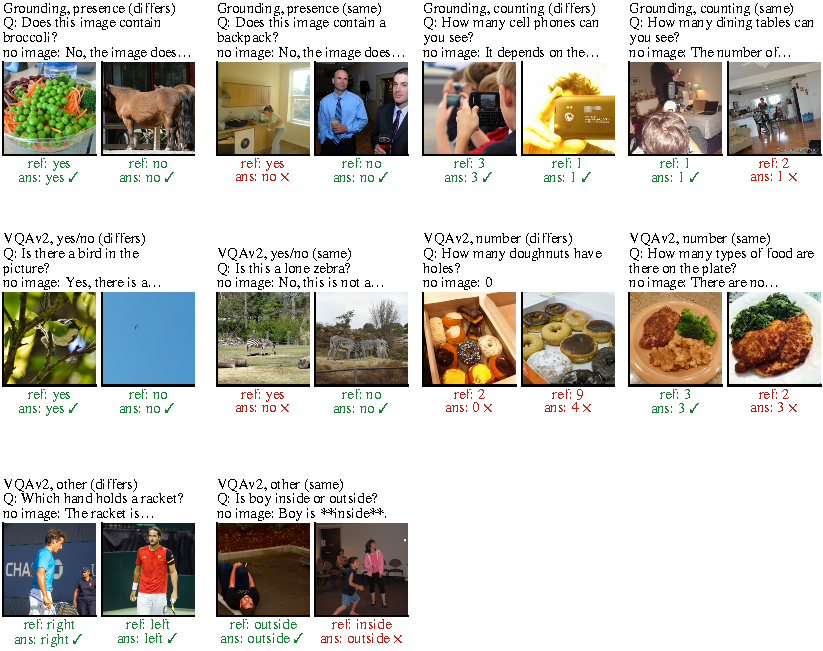
\includegraphics[width=\textwidth,height=0.85\textheight,keepaspectratio]{figs/task2/figA1_qualitative_all.pdf}
  \caption{\todo{Figure title.} \todo{1--2 sentences describing what is shown, including the example-selection rule.} \todo{Conclusion to draw.}}
  \label{fig:vlm-qualitative-all}
\end{figure}

% =====================================================================================================
\section{Test-Time Compute: Supplementary Results}
\label{app:ttc}

\subsection{Data, Answer Equivalence and Scorer Details}
\label{app:ttc-data}
\todo{Text.}
\begin{table}[t]
\centering
\small
\caption{Data and scorer details (all 1,000 questions per dataset).}
\label{tab:t3-data}
\begin{tabular}{llr}
\toprule
Dataset & Item & Value \\
\midrule
MATH (Qwen2.5-3B) & Rollout accuracy / NO\_ANSWER / capped & 66.3\% / 1.6\% / 1.6\% \\
 & Mean retained tokens per rollout & 648 \\
 & Splits (dev / held-out) & 200 / 800 \\
 & Math-Verify 0.9.0: comparisons hitting the time limit ($\to$ not equivalent) & 80 in 1 questions \\
MathVista (Qwen2.5-VL-3B) & Rollout accuracy / NO\_ANSWER / capped & 53.6\% / 15.4\% / 1.5\% \\
 & Mean retained tokens per rollout & 280 \\
 & Splits (dev / held-out) & 200 / 800 \\
 & MathVista metadata (testmini.json) SHA-256 & ab0148dca9d401c3… \\
\bottomrule
\end{tabular}
\end{table}


\subsection{Scorer Sensitivity}
\label{app:ttc-sensitivity}
\todo{Text.}
\begin{table}[t]
\centering
\small
\caption{MathVista scorer sensitivity (held-out accuracy, \%). Official: MathVista's answer-type / precision rules. Lenient (sensitivity check only): units, spacing commands, \$, degree / percent signs and thousands separators removed before those rules, for grouping and grading alike.}
\label{tab:t3-sensitivity}
\begin{tabular}{lrrrr}
\toprule
Method & Official N=8 & Lenient N=8 & Official N=32 & Lenient N=32 \\
\midrule
FirstAns & 53.6 & 54.2 & 53.6 & 54.2 \\
Self-consistency & 59.9 & 60.5 & 61.7 & 62.5 \\
Max mean log-prob & 51.9 & 52.7 & 48.1 & 49.0 \\
Max self-certainty & 54.8 & 55.6 & 54.6 & 55.6 \\
Self-certainty + RWC & 60.0 & 60.8 & 62.5 & 63.4 \\
Shortest (length control) & 54.6 & 54.9 & 53.8 & 54.1 \\
Max vision & 54.3 & 54.8 & 53.6 & 54.1 \\
Vision + RWC & 60.1 & 60.7 & 62.9 & 63.6 \\
Max VisConf & 56.3 & 56.8 & 57.8 & 58.1 \\
VisConf + RWC & 60.8 & 61.4 & 63.1 & 63.9 \\
Max VisConf (tokenwise) & 55.7 & 56.2 & 56.2 & 56.8 \\
VisConf tokenwise + RWC & 60.9 & 61.5 & 62.6 & 63.5 \\
NO\_ANSWER rate (rollouts) & 15.4 & 13.5 &  &  \\
Oracle coverage & 82.7 & 83.1 & 89.5 & 89.9 \\
\bottomrule
\end{tabular}
\end{table}


\subsection{All Selection Rules at All Budgets}
\label{app:ttc-curves}
\todo{Text.}
\begin{table}[t]
\centering
\small
\caption{MATH (Qwen2.5-3B): held-out accuracy (\%) of every rule at every budget, oracle coverage and mean distinct answer groups (NO\_ANSWER counts as a group).}
\label{tab:t3-curves-math}
\begin{tabular}{>{\raggedright\arraybackslash}p{3.4cm}rrrrrrr}
\toprule
Method & N=1 & N=2 & N=4 & N=8 & N=16 & N=32 & Tokens @32 \\
\midrule
FirstAns & 64.4 & 64.4 & 64.4 & 64.4 & 64.4 & 64.4 & 670 \\
Self-consistency & 64.4 & 64.4 & 69.2 & 71.8 & 73.1 & 73.8 & 21347 \\
Max mean log-prob & 64.4 & 65.8 & 67.2 & 67.5 & 66.4 & 64.0 & 21347 \\
Max self-certainty & 64.4 & 66.8 & 68.8 & 70.1 & 70.7 & 70.6 & 21347 \\
Self-certainty + RWC & 64.4 & 66.8 & 69.7 & 72.9 & 74.6 & 75.5 & 21347 \\
Shortest (length control) & 64.4 & 65.3 & 65.2 & 64.6 & 63.2 & 62.4 & 21347 \\
Oracle coverage & 64.4 & 72.5 & 79.1 & 84.3 & 88.4 & 91.4 & – \\
Distinct answer groups & 1.00 & 1.37 & 1.93 & 2.74 & 4.00 & 5.90 & – \\
\bottomrule
\end{tabular}
\end{table}

\begin{table}[t]
\centering
\small
\caption{MathVista (Qwen2.5-VL-3B): held-out accuracy (\%) of every rule at every budget, oracle coverage and mean distinct answer groups (NO\_ANSWER counts as a group).}
\label{tab:t3-curves-mathvista}
\begin{tabular}{lrrrrrrr}
\toprule
Method & N=1 & N=2 & N=4 & N=8 & N=16 & N=32 & Tokens @32 \\
\midrule
FirstAns & 53.6 & 53.6 & 53.6 & 53.6 & 53.6 & 53.6 & 278 \\
Self-consistency & 53.6 & 53.6 & 57.8 & 59.9 & 60.9 & 61.7 & 8898 \\
Max mean log-prob & 53.6 & 54.3 & 53.2 & 51.9 & 50.5 & 48.1 & 8898 \\
Max self-certainty & 53.6 & 54.7 & 55.0 & 54.8 & 55.0 & 54.6 & 8898 \\
Self-certainty + RWC & 53.6 & 54.7 & 56.8 & 60.0 & 61.3 & 62.5 & 8898 \\
Shortest (length control) & 53.6 & 55.0 & 55.2 & 54.6 & 54.3 & 53.8 & 8898 \\
Max vision & 53.6 & 54.3 & 54.5 & 54.3 & 54.0 & 53.6 & 8898 \\
Vision + RWC & 53.6 & 54.3 & 56.5 & 60.1 & 61.2 & 62.9 & 8898 \\
Max VisConf & 53.6 & 55.4 & 56.2 & 56.3 & 56.7 & 57.8 & 8898 \\
VisConf + RWC & 53.6 & 55.4 & 57.7 & 60.8 & 61.8 & 63.1 & 8898 \\
Max VisConf (tokenwise) & 53.6 & 55.4 & 55.9 & 55.7 & 55.7 & 56.2 & 8898 \\
VisConf tokenwise + RWC & 53.6 & 55.4 & 57.5 & 60.9 & 61.7 & 62.6 & 8898 \\
Oracle coverage & 53.6 & 66.0 & 75.9 & 82.7 & 87.1 & 89.5 & – \\
Distinct answer groups & 1.00 & 1.42 & 1.92 & 2.51 & 3.18 & 3.94 & – \\
\bottomrule
\end{tabular}
\end{table}

\begin{figure}[!htbp]
  \centering
  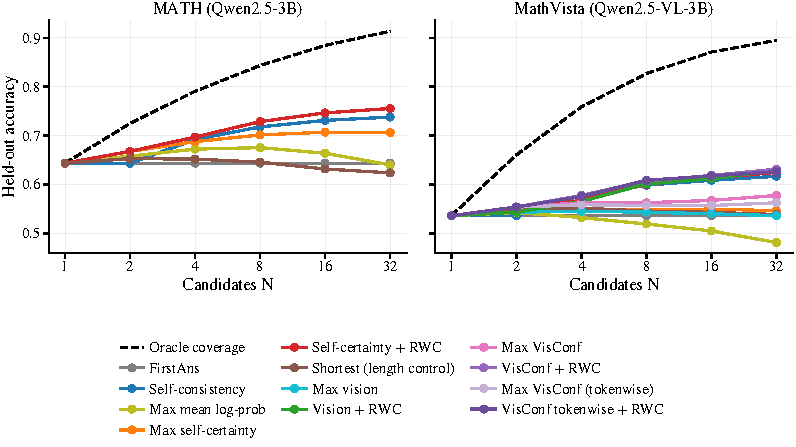
\includegraphics[width=\textwidth,height=0.85\textheight,keepaspectratio]{figs/task3/figA1_all_methods.pdf}
  \caption{\todo{Figure title.} \todo{1--2 sentences describing what is shown.} \todo{Conclusion to draw.}}
  \label{fig:ttc-all-methods}
\end{figure}

\subsection{Controlled Comparisons of Scores and Aggregation}
\label{app:ttc-bootstrap}
\todo{Text.}
\begin{table}[t]
\centering
\small
\caption{Controlled comparisons (pp, paired question-level bootstrap, 1,000 resamples): same aggregation with a different score, or the same score with a different aggregation.}
\label{tab:t3-boot}
\begin{tabular}{llrrrrr}
\toprule
Dataset & Comparison & N=2 & N=4 & N=8 & N=16 & N=32 \\
\midrule
MATH & Max self-certainty $-$ Max mean log-prob & +1.0 [+0.4, +1.6] & +1.5 [+0.6, +2.6] & +2.6 [+1.3, +3.9] & +4.3 [+2.8, +6.0] & +6.6 [+4.2, +9.1] \\
MATH & Self-consistency $-$ FirstAns & +0.0 [+0.0, +0.0] & +4.8 [+4.0, +5.6] & +7.4 [+6.4, +8.5] & +8.8 [+7.4, +10.1] & +9.4 [+7.8, +11.1] \\
MATH & Self-certainty + RWC $-$ Max self-certainty & +0.0 [+0.0, +0.0] & +0.9 [+0.5, +1.3] & +2.7 [+1.8, +3.7] & +4.0 [+2.5, +5.3] & +4.9 [+2.8, +7.2] \\
MathVista & Max self-certainty $-$ Max mean log-prob & +0.5 [-0.1, +1.1] & +1.8 [+0.8, +2.8] & +2.9 [+1.5, +4.2] & +4.5 [+2.5, +6.4] & +6.5 [+3.5, +9.6] \\
MathVista & Max VisConf $-$ Max self-certainty & +0.7 [-0.1, +1.4] & +1.2 [+0.2, +2.2] & +1.5 [-0.0, +3.0] & +1.8 [-0.3, +3.8] & +3.1 [-0.1, +6.2] \\
MathVista & Max VisConf $-$ Max vision & +1.1 [+0.4, +1.7] & +1.7 [+0.7, +2.7] & +1.9 [+0.7, +3.2] & +2.7 [+1.0, +4.5] & +4.1 [+1.1, +7.2] \\
MathVista & Max VisConf (tokenwise) $-$ Max VisConf & -0.0 [-0.4, +0.3] & -0.4 [-0.9, +0.1] & -0.5 [-1.2, +0.1] & -1.1 [-1.9, -0.1] & -1.5 [-3.2, +0.4] \\
MathVista & Self-consistency $-$ FirstAns & +0.0 [+0.0, +0.0] & +4.2 [+3.2, +5.0] & +6.3 [+5.1, +7.4] & +7.3 [+5.8, +8.8] & +8.1 [+6.2, +10.0] \\
MathVista & Self-certainty + RWC $-$ Max self-certainty & +0.0 [+0.0, +0.0] & +1.8 [+1.1, +2.4] & +5.3 [+4.1, +6.5] & +6.3 [+4.5, +8.2] & +7.9 [+4.7, +10.9] \\
MathVista & VisConf + RWC $-$ Max VisConf & +0.0 [+0.0, +0.0] & +1.5 [+0.8, +2.1] & +4.5 [+3.3, +5.6] & +5.1 [+3.3, +6.8] & +5.4 [+2.5, +8.1] \\
MathVista & VisConf + RWC $-$ Self-certainty + RWC & +0.7 [-0.1, +1.4] & +1.0 [+0.3, +1.7] & +0.7 [-0.1, +1.6] & +0.6 [-0.4, +1.4] & +0.6 [-0.6, +2.0] \\
MathVista & VisConf tokenwise + RWC $-$ VisConf + RWC & -0.0 [-0.4, +0.3] & -0.2 [-0.5, +0.1] & +0.1 [-0.3, +0.5] & -0.1 [-0.5, +0.3] & -0.5 [-1.1, +0.0] \\
MathVista & Vision + RWC $-$ Max vision & +0.0 [+0.0, +0.0] & +2.0 [+1.3, +2.7] & +5.8 [+4.5, +7.1] & +7.2 [+5.2, +9.1] & +9.2 [+6.1, +12.4] \\
\bottomrule
\end{tabular}
\end{table}


\subsection{Signal Analysis Details}
\label{app:ttc-signals}
\todo{Text.}
% moved from the main body to save space
\begin{table}[t]
\centering
\small
\caption{Signal analysis at N = 32 (held-out). Quartile $\Delta$: correctness of a question's top-quartile rollouts by the score minus its bottom quartile, averaged over all questions / questions with mixed correctness. Spearman: within-question rank correlation with rollout length, median [IQR]. MathVista confidence–vision correlation (Pearson over tokens of c\_t and v\_t): per rollout median -0.21 [IQR -0.33, -0.07], n = 25,572; per-question mean -0.21. Tokenwise − trajectory fusion equals Cov\_t(c, v) up to 1.8e-08 (numerical check).}
\label{tab:t3-signals}
\begin{tabular}{lrrrr}
\toprule
Score & MATH quartile $\Delta$ (all / mixed), pp & MathVista quartile $\Delta$ (all / mixed), pp & MATH Spearman with length & MathVista Spearman with length \\
\midrule
Self-certainty K & +12.0 / +20.4 & +3.5 / +4.4 & -0.18 [-0.44, +0.07] & +0.38 [+0.12, +0.60] \\
Mean log-prob L & +7.8 / +13.4 & +1.6 / +2.0 & +0.24 [-0.03, +0.51] & +0.38 [+0.12, +0.59] \\
Shortness (−length) & +4.6 / +7.8 & +4.1 / +5.1 & – & – \\
Vision V & – & +3.8 / +4.8 & – & -0.79 [-0.89, -0.62] \\
Calibrated confidence C & – & +3.8 / +4.8 & – & +0.37 [+0.12, +0.60] \\
VisConf Z = V·C & – & +7.4 / +9.3 & – & -0.35 [-0.57, -0.08] \\
Tokenwise mean(c·v) & – & +7.2 / +9.1 & – & -0.41 [-0.61, -0.13] \\
\bottomrule
\end{tabular}
\end{table}


\subsection{Token-Level Signal Trajectories}
\label{app:ttc-trajectories}
\todo{Text.}
\begin{figure}[!htbp]
  \centering
  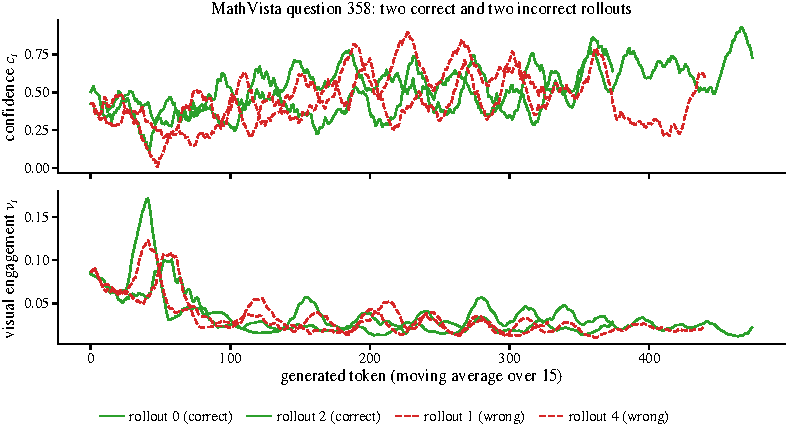
\includegraphics[width=\textwidth,height=0.85\textheight,keepaspectratio]{figs/task3/figA3_trajectories.pdf}
  \caption{\todo{Figure title.} \todo{1--2 sentences describing what is shown, including how the trajectories were selected.} \todo{Conclusion to draw.}}
  \label{fig:ttc-trajectories}
\end{figure}

\subsection{Adaptive Stopping: Development Grids and Stopping Behaviour}
\label{app:ttc-adaptive}
\todo{Text.}
% Long table: may need to be split or converted to longtable if it overflows the page.
\begin{table}[t]
\centering
\small
\caption{Development-set grids for adaptive stopping (eligible = within 1 pp of fixed-32 self-consistency).}
\label{tab:t3-grid}
\begin{tabular}{llrrrrrl}
\toprule
Dataset & Family & τ & γ & \makecell{Dev\\accuracy \%} & \makecell{Dev tokens\\/ q.} & Dev rollouts & Eligible \\
\midrule
MATH & fixed32 & – & – & 82.5 & 18322 & 32.0 & yes \\
MATH & agreement & 0.5 & – & 81.4 & 5053 & 6.6 & no \\
MATH & agreement & 0.625 & – & 82.6 & 7089 & 9.2 & selected \\
MATH & agreement & 0.75 & – & 82.6 & 7717 & 10.1 & yes \\
MATH & agreement & 0.875 & – & 82.6 & 9980 & 13.6 & yes \\
MATH & agreement & 1.0 & – & 82.6 & 10848 & 15.2 & yes \\
MATH & fixed32 & – & – & 82.5 & 18322 & 32.0 & yes \\
MATH & quality & 0.5 & 0.0 & 82.2 & 5480 & 7.2 & selected \\
MATH & quality & 0.5 & 0.1 & 82.2 & 5664 & 7.4 & yes \\
MATH & quality & 0.5 & 0.25 & 82.1 & 6009 & 7.9 & yes \\
MATH & quality & 0.5 & 0.5 & 82.2 & 7018 & 9.3 & yes \\
MATH & quality & 0.625 & 0.0 & 82.7 & 7129 & 9.2 & yes \\
MATH & quality & 0.625 & 0.1 & 82.7 & 7249 & 9.4 & yes \\
MATH & quality & 0.625 & 0.25 & 82.6 & 7293 & 9.5 & yes \\
MATH & quality & 0.625 & 0.5 & 82.5 & 7811 & 10.3 & yes \\
MATH & quality & 0.75 & 0.0 & 82.7 & 7756 & 10.2 & yes \\
MATH & quality & 0.75 & 0.1 & 82.7 & 7928 & 10.4 & yes \\
MATH & quality & 0.75 & 0.25 & 82.6 & 7941 & 10.5 & yes \\
MATH & quality & 0.75 & 0.5 & 82.5 & 8242 & 11.0 & yes \\
MATH & quality & 0.875 & 0.0 & 82.6 & 9980 & 13.6 & yes \\
MATH & quality & 0.875 & 0.1 & 82.6 & 9980 & 13.6 & yes \\
MATH & quality & 0.875 & 0.25 & 82.6 & 9980 & 13.6 & yes \\
MATH & quality & 0.875 & 0.5 & 82.6 & 9980 & 13.6 & yes \\
MATH & quality & 1.0 & 0.0 & 82.6 & 10848 & 15.2 & yes \\
MATH & quality & 1.0 & 0.1 & 82.6 & 10848 & 15.2 & yes \\
MATH & quality & 1.0 & 0.25 & 82.6 & 10848 & 15.2 & yes \\
MATH & quality & 1.0 & 0.5 & 82.6 & 10848 & 15.2 & yes \\
MathVista & fixed32 & – & – & 64.2 & 9217 & 32.0 & yes \\
MathVista & agreement & 0.5 & – & 63.6 & 3807 & 9.7 & selected \\
MathVista & agreement & 0.625 & – & 64.5 & 5301 & 14.0 & yes \\
MathVista & agreement & 0.75 & – & 64.4 & 5704 & 15.3 & yes \\
MathVista & agreement & 0.875 & – & 64.2 & 7098 & 20.3 & yes \\
MathVista & agreement & 1.0 & – & 64.2 & 7455 & 22.1 & yes \\
MathVista & fixed32 & – & – & 64.2 & 9217 & 32.0 & yes \\
MathVista & quality & 0.5 & 0.0 & 64.0 & 4199 & 10.9 & selected \\
MathVista & quality & 0.5 & 0.1 & 64.0 & 4452 & 11.7 & yes \\
MathVista & quality & 0.5 & 0.25 & 64.0 & 4750 & 12.7 & yes \\
MathVista & quality & 0.5 & 0.5 & 64.2 & 5523 & 15.2 & yes \\
MathVista & quality & 0.625 & 0.0 & 64.5 & 5373 & 14.2 & yes \\
MathVista & quality & 0.625 & 0.1 & 64.4 & 5481 & 14.6 & yes \\
MathVista & quality & 0.625 & 0.25 & 64.3 & 5530 & 14.8 & yes \\
MathVista & quality & 0.625 & 0.5 & 64.3 & 5917 & 16.2 & yes \\
MathVista & quality & 0.75 & 0.0 & 64.3 & 5785 & 15.6 & yes \\
MathVista & quality & 0.75 & 0.1 & 64.2 & 5917 & 16.0 & yes \\
MathVista & quality & 0.75 & 0.25 & 64.2 & 5921 & 16.1 & yes \\
MathVista & quality & 0.75 & 0.5 & 64.5 & 6145 & 17.0 & yes \\
MathVista & quality & 0.875 & 0.0 & 64.2 & 7098 & 20.3 & yes \\
MathVista & quality & 0.875 & 0.1 & 64.2 & 7098 & 20.3 & yes \\
MathVista & quality & 0.875 & 0.25 & 64.2 & 7098 & 20.3 & yes \\
MathVista & quality & 0.875 & 0.5 & 64.2 & 7098 & 20.3 & yes \\
MathVista & quality & 1.0 & 0.0 & 64.2 & 7455 & 22.1 & yes \\
MathVista & quality & 1.0 & 0.1 & 64.2 & 7455 & 22.1 & yes \\
MathVista & quality & 1.0 & 0.25 & 64.2 & 7455 & 22.1 & yes \\
MathVista & quality & 1.0 & 0.5 & 64.2 & 7455 & 22.1 & yes \\
\bottomrule
\end{tabular}
\end{table}

\begin{figure}[!htbp]
  \centering
  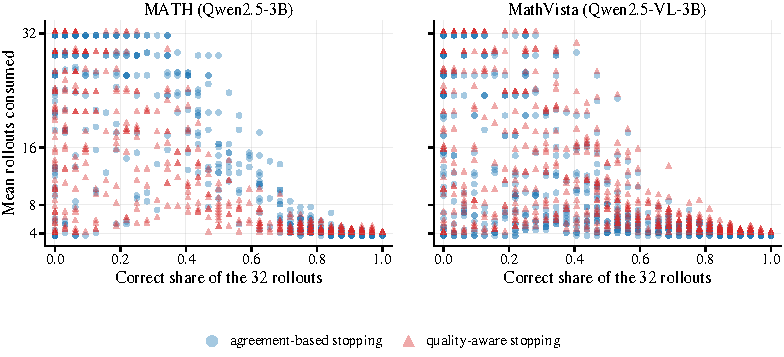
\includegraphics[width=\textwidth,height=0.85\textheight,keepaspectratio]{figs/task3/figA2_stopping_vs_correct.pdf}
  \caption{\todo{Figure title.} \todo{1--2 sentences describing what is shown.} \todo{Conclusion to draw.}}
  \label{fig:ttc-stopping}
\end{figure}

\end{document}
